\documentclass{article}
\usepackage[T1]{fontenc}
\usepackage{microtype}
\usepackage{graphicx,booktabs}
\usepackage{amsmath,amssymb}
\usepackage{tikz}
\usetikzlibrary{arrows.meta,positioning,calc,fit,backgrounds}
\usepackage{pgfplots}
\pgfplotsset{compat=1.18}
\usepackage{xurl}
\usepackage[hyperfootnotes=false]{hyperref}
\newcommand{\theHalgorithm}{\arabic{algorithm}}
\usepackage{mlsys2025}
\definecolor{answerblue}{HTML}{31688E}
\definecolor{updatepurple}{HTML}{7860A0}
\definecolor{freshorange}{HTML}{CE8A32}
\definecolor{passgreen}{HTML}{3B8C71}
\definecolor{formatamber}{HTML}{E3B65D}
\definecolor{failgray}{HTML}{B6BEC8}
\hypersetup{hypertexnames=false,pdftitle={From Resource Savings to Useful Answers},pdfsubject={Research characterization draft. Official blind-review template}}
\mlsystitlerunning{From Resource Savings to Useful Answers}
\begin{document}
\twocolumn[
\mlsystitle{From Resource Savings to Useful Answers:\\Characterizing Shared ARM Inference and Document Updates}
\begin{mlsysauthorlist}
\mlsysauthor{Anonymous Authors}{anon}
\end{mlsysauthorlist}
\mlsysaffiliation{anon}{Anonymous Institution}
\mlsyscorrespondingauthor{Anonymous Author}{anon.email@domain.com}
\mlsyskeywords{edge inference, resource contention, RAG, grounded answers, experimental methodology}
\vskip 0.3in
\begin{abstract}
A document assistant must answer questions while new documents are indexed on the same machine. We present an evaluation methodology and an implemented framework that schedules concurrent jobs and independent requests, enforces CPU allocations, links index publication to retrieval, and records phase times, resource use and answer checks. We evaluate Qwen2.5-14B-Instruct in Q4\_K\_M on a Raspberry Pi 5 in 75 cells covering isolated controls, matched update episodes and predictions fixed before testing other cases. Reserving two cores improves ingestion (13.8 to 7.0\,s) but slows the long-prompt answer (174.3 to 246.4\,s), mainly in prefill. Publication precedes slot release in all concurrent E2/E3 episodes (36/36), while prediction error is comparable to a simple baseline (MAE 22.22\,s versus 21.48\,s). The framework exposes the cost of fixed reservations and separates timing gains from answer validity, with independent semantic review still pending.
\end{abstract}
]
\section{Introduction}
A document assistant must keep answering questions as its sources change.
New documents need to become searchable, and answers need to be supported by
the retrieved text. Both requirements have been studied in search and RAG
systems \citep{freshdiskann,metis,alce}. When ingestion and LLM inference run
on the same small machine, they also compete for CPU time and memory.

There are several ways to share those resources. Delaying an update gives
inference more time but makes users wait for new information. Reserving cores
for ingestion can help it finish sooner. A fixed reservation, however, can
continue to limit inference after embedding has finished. We study how these
choices affect the whole request. Does an earlier index update lead to an
earlier answer, or does the cost appear elsewhere?

Recent measurement studies ask similar questions about other parts of LLM
serving. Breaking the Ice identifies the stages responsible for startup time.
\emph{Speculative Decoding: Performance or Illusion?} checks whether speedups
seen in prototypes hold in a production engine \citep{breakingice,specillusion}.
\emph{Beyond the Buzz} studies how workloads and configurations change the
benefits of disaggregation \citep{beyondbuzz}. These works show the value of
measuring where an optimization saves time and where it adds cost.

Scheduling systems already account for different inference phases.
Sarathi-Serve uses chunked prefills, DistServe separates prefill and decode
resources, and SuperInfer coordinates scheduling with KV transfers
\citep{sarathi,distserve,superinfer}. METIS adapts RAG configuration and
scheduling to meet quality requirements \citep{metis}. We build on this
perspective with an evaluation framework for CPU allocation, document publication and
answer completion on a Raspberry Pi 5. We evaluate fixed allocations.
We do not introduce a new adaptive scheduler.

Our method has three steps. We first run inference and ingestion separately
and together, recording phase times and checking which CPUs each thread can
use. We then run matched application episodes with different update policies
and request arrival times. Finally, we fix timing predictions before testing
them on other documents and arrivals. At every step, we check answer quality,
citations and the retrieved version separately from response time.
Section~\ref{sec:problem} defines the evaluation steps.

We run the full Qwen2.5-14B-Instruct model in Q4\_K\_M on a Raspberry Pi 5
with 16 GB RAM, alongside the MiniLM document worker. This gives a concrete
setting for studying contention on a small CPU system. The 27 diagnostic
cells show a clear trade-off. Reserving two
cores for ingestion almost halves update time under concurrency, but increases
the long-prompt answer time from 174.3 to 246.4\,s. Most of the extra time is in
prefill. In 36 application episodes, publication finishes before current
inference under both concurrent policies, even when the index is rebuilt.
The fixed partition also slows the next request. In 12 further episodes, the
predictions correctly rank the two policies in six pairs, but their accuracy
is no better than a simple baseline added after the experiment.

Our contribution is an evaluation methodology and its implemented framework.
We built the controller for CPU allocation and independent request arrivals,
connected versioned document publication to retrieval and inference, and added
phase measurements, resource sampling and answer checks. The framework retains
inputs, outputs and prediction hashes so each comparison can be traced to its
configuration. These components make the allocation trade-offs measurable with
existing runtimes. Earlier precision, backend and QA experiments provide
separate controls rather than extra repetitions of the 75 cells. Our documents
and arrivals are controlled cases, not production traces. Dynamic core
reassignment and independent human review of answer correctness remain open.

\section{Related Work: Evaluation and Resource Sharing}
\subsection{Measurement Studies}
Breaking the Ice divides vLLM startup into six stages, measures how their costs
change with model and system parameters, and builds a predictor
\citep{breakingice}. \citet{specillusion} test speculative decoding in vLLM
across workloads, models and batch settings. They relate measured execution
times to acceptance behavior and speedup bounds. These studies support using
phase measurements and strong runtime controls. Empirical evaluation of
autoregressive inference on resource-constrained Raspberry Pi 5 nodes also
provides context for the platform used here \citep{daian2026rpi}.
We apply this approach to
ingestion and inference, check answers and retrieved versions, and fix timing
predictions before testing other cases. Our study covers one 14B model and
controlled documents. Its predictor does not show an accuracy advantage.

\emph{Beyond the Buzz} explores how workloads and configurations affect
prefill/decode disaggregation \citep{beyondbuzz}. ProfInfer uses eBPF probes to
inspect inference in engines such as llama.cpp \citep{profinfer}. These Industry
Track studies provide context for our design and measurements. ProfInfer also
shows why operator and phase behavior matter. Our process and thread samples
and server timers give less detail. They do not separate cache from bandwidth
causes. We have not run either system as a competitor in our experiments.

\subsection{Scheduling and CPU Allocation}
Sarathi-Serve uses chunked prefills and stall-free batching to reduce
prefill/decode interference. DistServe places the two phases on separate
resources and tunes allocation for their latency requirements
\citep{sarathi,distserve}. SuperInfer combines scheduling with KV transfers on
Superchips to meet response time targets \citep{superinfer}. These systems
already account for phase demand. We study the effect of a fixed CPU reservation
that remains after ingestion ends. We do not test a scheduler that returns
idle cores to inference or show that such a scheduler would be new.

PagedAttention reduces KV fragmentation and supports sharing. FlexGen places
work across GPU, CPU and disk to improve throughput with limited GPU memory
\citep{pagedattention,flexgen}. Their objectives differ from the time to finish
one interactive request. ServerlessLLM combines checkpoint loading, migration
and scheduling based on startup cost \citep{serverlessllm}. This motivates
reporting readiness separately from warm requests. Our execution baseline is
the frozen ARM llama.cpp server \citep{llamacpp}. Published GPU speedups do
not estimate what these systems would achieve within our CPU budget.

\subsection{Freshness and Answer Quality in RAG}
METIS adapts RAG configuration and scheduling to meet quality requirements
\citep{metis}. FreshDiskANN maintains a graph index under streaming updates
\citep{freshdiskann}. We study when a separately arriving question can use a
published update while inference shares the same resources. Our MiniLM worker
uses an exact dense index. We do not propose an ANN method or compare against
implementations of METIS or FreshDiskANN.

ALCE evaluates answer correctness and citation quality separately. SQuAD2
includes questions that cannot be answered from the supplied text
\citep{alce,squad2}. These works motivate our separate checks for answers,
citations and versions. The earlier 24-article test includes unanswerable
questions. E2/E3 use six answerable questions under different configurations.
An exact-match failure alone does not show a hallucination. Human review is
still needed to assess meaning and support.

\subsection{Earlier Mechanism Controls}
GPTQ and AWQ are quantization methods \citep{gptq,awq}. DroidSpeak and ElastKV
reuse KV across model variants or precisions and selectively recompute state
\citep{droidspeak,elastkv}. Attention omission has also been studied
\citep{attentiondrop}. EdgeShard addresses placement across devices, while
PipeLive supports live pipeline reconfiguration \citep{edgeshard,pipelive}.
These works provide context for our earlier precision, state and execution
controls. The E1--E3 evaluation instead centers on resource allocation.

Our contribution is the evaluation framework and the measured relationship between CPU
sharing, phase costs, fixed reservations and answer timing. All concurrent
cases remain limited by the inference slot, and the predictor performs about
as well as a simple baseline added later. The findings identify problems to
test further. They do not establish a first general evaluation method,
a new scheduler or superiority over the systems discussed here.

\section{Evaluation Methodology}
\label{sec:problem}
Our methodology follows the effect of an inference change from resource use
to the final answer. It separates four questions, summarized in
Table~\ref{tab:research-questions}. The implemented workflow is shown in
Figure~\ref{fig:research-system}.

\begin{table}[!htb]
\caption{Research questions and the evidence used to answer them.}
\label{tab:research-questions}
\centering
\begin{tabular}{@{}p{.7cm}p{3.6cm}p{2.7cm}@{}}
\toprule
 & Question & Evidence\\
\midrule
RQ1 & Does released memory let concurrent work progress? & Process and node memory, update progress\\[3pt]
RQ2 & Do backend settings and CPU allocations improve execution? & Standard backend, prefill and generation times\\[3pt]
RQ3 & Do individual answers and citations remain valid? & Paired QA checks, raw answers and citations\\[3pt]
RQ4 & Does a change improve the full episode, and can its timing be predicted? & Publication, request completion and prediction errors\\
\bottomrule
\end{tabular}
\end{table}

\begin{figure*}[t]
\centering
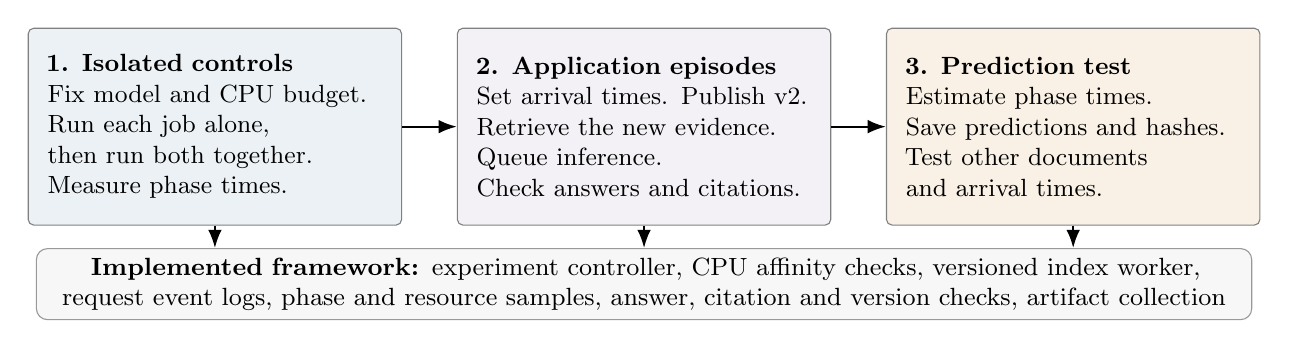
\begin{tikzpicture}[font=\small,>=Latex,
 methodbox/.style={draw=black!50,rounded corners=2pt,align=left,text width=4.25cm,minimum height=2.5cm,inner sep=7pt},
 flow/.style={->,line width=.8pt}]
\node[methodbox,fill=answerblue!9] (one) at (0,0) {\textbf{1. Isolated controls}\\
Fix model and CPU budget.\\
Run each job alone,\\then run both together.\\Measure phase times.};
\node[methodbox,fill=updatepurple!9] (two) at (5.45,0) {\textbf{2. Application episodes}\\
Set arrival times. Publish v2.\\
Retrieve the new evidence.\\Queue inference.\\Check answers and citations.};
\node[methodbox,fill=freshorange!12] (three) at (10.9,0) {\textbf{3. Prediction test}\\
Estimate phase times.\\Save predictions and hashes.\\
Test other documents\\and arrival times.};
\draw[flow] (one)--(two);\draw[flow] (two)--(three);
\node[draw=black!40,rounded corners,align=center,text width=15.2cm,minimum height=.9cm,fill=black!3] (impl) at (5.45,-2.0)
{\textbf{Implemented framework:} experiment controller, CPU affinity checks, versioned index worker,\\
request event logs, phase and resource samples, answer, citation and version checks, artifact collection};
\draw[flow] (one.south)--(one.south |- impl.north);
\draw[flow] (two.south)--(impl.north);
\draw[flow] (three.south)--(three.south |- impl.north);
\end{tikzpicture}
\caption{The evaluation workflow and the components we implemented. E1 applies
step 1, E2 applies step 2 and E3 applies step 3. Inputs and resource budgets
are fixed for each matched comparison. Timing and answer checks remain separate,
and prediction errors are retained without refitting.}
\label{fig:research-system}
\end{figure*}


\subsection{Evaluation Steps}
\textbf{1. Establish isolated controls.} Fix the model, backend, inputs and
resource budget. Run ingestion and inference alone, then together. Record
startup, memory use and phase times. A standard backend provides the execution
reference so that poor settings are not mistaken for an optimization opportunity.

\textbf{2. Measure the application episode.} Start an update while the current
request runs. Schedule a new question independently, wait for its required index
version, retrieve evidence and submit the request. Compare policies on matched
inputs and arrivals. Keep answer, citation and version checks separate from
latency. This step connects a local resource change to the user's request.

\textbf{3. Test the explanation.} Estimate phase durations from the earlier
runs, save the predictions and their hashes, then evaluate other document and
arrival combinations. Retain errors and failed answers without changing the
policy, labels or predictor to improve the result. E1, E2 and E3 instantiate
these steps with the experiments defined in Section~\ref{sec:budget}.

\subsection{Episode Measurements}
The current request keeps its original context while the update worker chunks
and embeds changed documents and publishes v2. A new question must retrieve
and cite the new evidence. Let $T_c$ be current completion, $T_p$ publication
and $T_f$ new-answer completion, measured from update arrival. We report all
three times and latency from the new question's own arrival. Finishing
generation does not mean that an answer passes the quality checks.

In the earlier sequential control, the new request starts after both current
completion and publication. Its timing is
\begin{equation}
T_f=\max(T_c,T_p)+T_{\mathrm{retrieve}}+T_{\mathrm{new\ request}}.
\label{eq:critical-path}
\end{equation}
For independent arrivals, retrieval waits for arrival and publication. The new
request then queues for the inference slot. The E3 estimate follows this order,
using measured phase durations. The order is a property of the experiment.
Whether the phase estimates predict other cases is tested separately.

We have no application SLA or independently reviewed utility score. We therefore
report timing and answer checks directly, without a weighted score chosen after
the results. Correct answers, supported citations, relevant versions and
abstention are assessed as separate outcomes.

\subsection{Implemented Components}
\label{sec:mechanisms}
We implemented an experiment controller that starts isolated and concurrent
jobs, schedules request arrivals independently and enforces the CPU allocation
for each process. It checks thread affinity during execution, saves timing
and resource samples, and collects outputs before removing its experiment pod.

The controller connects inference to a document worker that reuses unchanged
embeddings, publishes index versions atomically and retrieves evidence for the
new request. Separate checks record answer agreement, citation validity and
the retrieved version. The framework also saves predictions and their hashes
before the final timing test, along with the inputs, configuration and source
hashes needed to trace each result. These are the components we built around
llama.cpp, MiniLM and existing data and scoring tools. We do not claim that
these general capabilities were absent from all previous systems.

\paragraph{Earlier Distributed Precision Control}
A separate four-node pilot changes only stage 0 of Qwen2.5-14B between existing
Q4\_K\_M/Q3\_K\_M artifacts. At a token boundary it exports KV, destroys and
unmaps the old executor, loads the target, imports state and checks re-export
integrity. Replaying the full prefix through all stages checks target-model accuracy. This validates
a transition path rather than a new quantizer or selective repair algorithm.
The detailed lifecycle is retained in the separate artifact appendix.

\paragraph{CPU Execution and Fixed Attention Omission}
The later monolithic worker keeps the full Q4\_K\_M model loaded, distinguishes
readiness from request timing and clears KV before each request. Four threads
serve prefill and two serve decode, with an explicit prompt boundary so a
singleton prefill tail remains in the prefill phase. Each logical frame contains 64 tokens. The physical microbatch size controls
how the graph is split. Runtime repacking
changes the CPU weight layout for existing quantized kernels \citep{llamacpp}.
It neither changes the GGUF file nor introduces a new quantization method.

We test raw microbatches of 2, 8, 32 and 64, and repacked microbatches of 2 and 64. Larger batches and
layout changes are opt-in approximate execution configurations: the raw-mb2
worker reproduces reference logits at 64/565 tokens, but that equality is not
assumed for other configurations. Repacking can increase startup and anonymous
memory, so those costs are measured separately from warm requests.

The fixed mask omits attention sublayers 39--42, including their Q/K/V/O
operations and KV writes, while retaining every FFN. The mask is constant
for a session. Online reactivation is not implemented: missing KV and changed
downstream states prevent treating it as a free reversible action. Attention
dropping is established prior work \citep{attentiondrop}. Residual similarity suggests candidate layers to omit. Answer checks determine
whether a configuration passes.

\paragraph{What Each Change Tests}
Precision changes target memory use. Batching and repacking target execution time.
Attention omission removes work at potential quality cost. Update deferral
protects the current request by delaying freshness. Each is evaluated at its
own endpoint before being connected to utility. A successful implementation,
a smaller process counter and an acceptable application outcome are different
claims. We implement no controller that jointly selects these actions online.


\section{Experimental Design}
\label{sec:methods}
\subsection{Experimental Setups}
\textbf{Distributed mechanism pilot.} Each of four ARM stage workers uses one compute thread. Activations pass through \texttt{kubectl exec}. Three
64-token synthetic cycles measure process and node memory after warmup. Three CoQA
conversations \citep{coqa}, with 458--513-token contexts and gold history,
compare Q4, static Q3 stage 0, retained transitions and full replay. Teacher
forcing and generation use separate passes with the same switch schedule.
This validates state handling. It does not measure production transport performance.

\textbf{Raspberry Pi 5 execution.} E1--E3 run on a Raspberry Pi 5 with
16 GB physical RAM and NVMe storage. Its four Cortex-A76 cores have a
2.4\,GHz maximum clock, dot-product and FP16 support and 2\,MiB shared L3.
The full Qwen2.5-14B-Instruct Q4\_K\_M model is approximately 8.79\,GB.
Inference is CPU-only, with no GPU. The container receives a four-CPU quota
and a 12-GiB memory safety cap. This cap is distinct from physical RAM and
is not a measured minimum deployment requirement. Governor
settings stay unchanged. Thermal and other variation are not fully eliminated.
The short and long prompts contain 184 and 565 tokens. Synthetic prefix tests
use 128, 256, 512 and 1024 tokens with cleared KV. These are length probes,
not four independent QA tasks.
Three cyclic repetitions produce descriptive medians, not confidence bounds.

\subsection{A Competitive Static Baseline}
We build an unmodified \texttt{llama-server} from the same frozen runtime
revision as the private worker (\texttt{838374375cb8}). It uses one slot, context 2048, logical batch
512, repacking, four prefill threads and two decode threads and no GPU. Four candidates
use physical batches of 64, 256 and 512 with F32 KV and flash attention off, plus batch
512 with F16 KV and flash-auto. This search covers four configurations and does not establish the best
possible backend. The F32 arms isolate batch size. The last arm
is a competitive configuration, not a single-variable causal ablation.

Selection uses only the existing supported short and long cases, three cyclic
repetitions each. Minimum median answer time among complete passing arms
selects the batch512/F16/flash-auto configuration. All configurations are fixed
before new-document inference. Explicit token IDs, greedy generation, repeat
penalty 1 and a 64-token cap match the private prototype. Prompt reuse is off.
Token and cache counters check for prefix reuse and truncation.
Requests start without reused prompt state. Production caching is outside
this comparison.

\subsection{QA on Separate Articles}
The subsequent cohort selects 24 distinct SQuAD2 article titles
\citep{squad2}, one paragraph and question per title, alternating 12 answerable and
12 unanswerable questions. Source order and a prospective 1200-token bound
select inputs without model outputs. An exact quoted-ID scan covers 4,997
prior local JSON/JSONL records, excluding an article if a question ID appears.
Exact normalized CoQA story duplicates are also excluded. The scan does not cover unlogged exposure, paraphrases or model pretraining. The
cohort is separate from tuning, not a broad confirmatory sample or a household
utility dataset. An earlier conservative CoQA preparation failed its cohort
availability gate before inference and was not relaxed retrospectively.

Each arm generates once per article after clearing KV. We retain official
SQuAD reference-based EM/F1, raw text and tokens, exact-reference agreement, citation
locator and EOS. The frozen automatic task pass requires a reference-exact
answer with the supplied source and chunk, or bare \texttt{unknown} without a
citation for an unanswerable case. Candidate admission checks for losses on
cases passed by standard. These checks measure reference matching and formatting. They do not replace
human assessment of meaning. A blinded review packet and separate key exist. Human review is pending.
Later inspection explains formatting failures while retaining the original scores.

\subsection{Defined Experiments}
\label{sec:budget}
\textbf{E1: diagnosis.} We run 27 cells in three cyclic blocks with the same
four-core budget. They include ingestion alone and two existing supported
prompts under inference alone, shared execution, a fixed 2+2 split and a fixed
3+1 split. Prefill and decode thread counts follow the LLM allocation. The
encoder receives two threads in 2+2 and one in 3+1. We set affinity before
creating threads and check it during each run. Warmup and v1 index preparation
are outside timing. Prompt KV reuse is off. These policies change both thread
counts and CPU placement, so they do not isolate cache or bandwidth effects.

\textbf{E2: application.} We run 36 episodes with three added articles, two
arrival offsets (0/90\,s), three policies (shared, 2+2, deferred) and two ways
of updating the index. Incremental publication embeds 82 new chunks. A rebuild
embeds the same complete 269-chunk v2 corpus in an empty staging index, then
switches the active pointer atomically. The old v1 remains readable during
the build. We do not pad the corpus to make updates slower.
The new request arrives at its scheduled time, waits for v2, retrieves the
top three passages and submits to the server. The old request may still occupy
the only inference slot. We record submission, first token and engine phase
timers. The engine does not expose the exact time a request leaves its queue.
The old request uses the same supplied context that passed the earlier checks.

\textbf{E3: timing test.} We use the next three articles, arrivals at 30/60\,s
and the two concurrent policies, giving 12 episodes. Before running them, we
use E2 incremental medians for each policy to predict current completion,
publication, retrieval and new-request service time. Engine prompt and
generation timers exclude queue waiting. The completion estimate is
$\max\{T_c,\max(T_a,T_p)+T_r\}+T_s$, where $T_a$ is arrival, $T_r$ is retrieval
and $T_s$ is service time. We save hashes of the parameters and predictions
and do not fit them again. These articles have appeared in earlier model
runs. They test timing on other cases, not semantic accuracy on unseen data.
An infrastructure failure interrupted E2 after 17 saved episodes. We retained
those episodes and ran the remaining 19 with the same experimental settings.


\subsection{Earlier Sequential Episode Control}
Before E1--E3 (Section~\ref{sec:budget}), four policies compare standard concurrent, standard deferred, full-prototype
concurrent and skip4-prototype concurrent. Three cyclic matched blocks add
three different answerable cohort documents to the existing real Git update
with 81 new chunks. These are three matched document episodes, not three
within-document replications. All policies receive the same snapshots per block.
There is no padding or artificial full-corpus reembedding.

Each episode builds fresh v1 outside timing and verifies absence of the new
source. The encoder is \texttt{sentence-transformers/all-MiniLM-L6-v2}.
It uses intra-op 2/inter-op 1, batch 4 and stable chunks of at most
256 encoder tokens. The current request starts when the update arrives and uses the supplied
context chosen in advance. The new request, after current completion and publication,
uses actual dense top-3 retrieval from v2. The gold passage is never substituted.
Current-query retrieval is not independently evaluated. The application score
checks the new source and version, the answer, and every citation against retrieved
locators. Failed answers remain in timing and quality records. No candidate
with a new-document regression can qualify for an automatic joint-benefit claim.

\subsection{Analysis Procedure}
For each matched case, we compare current-answer time, publication time and
new-answer latency. We report medians and paired differences without combining
different update modes or treating documents as repeated runs of one request.
We inspect prefill and generation separately to locate the cost of an allocation.
Answers that fail a check remain in both the timing record and the quality count.

For E3, we compare each saved prediction with its measured value and report
mean absolute error and relative error. We also check whether the predicted
policy order agrees with each matched pair. After E3, we add a simple baseline
using the E2 median total time for each policy. This is a later diagnostic,
not a comparison chosen before E3. No predictor is refitted.

\subsection{Records and Earlier Experiments}
Protocols, hashes of source and configuration files, outputs and failures are retained.
The final execution campaign contains 112 cells. The later validation contains
108 cells plus 12 application episodes. File-backed versus anonymous RSS,
process high-water marks and pod-lifetime peaks have different scopes. Page
ownership is not normalized. The standard package's first deployment missed
a shared library and stopped before inference. The corrected package was
verified on ARM before the measured run. Earlier transport failures and input
amendments remain in the record.

The earlier TinyLlama accounting and quality and CoQA switch-position protocols
remain separate in the appendix. Their original thresholds and verdicts are
not replaced by the later exploratory criteria. A read-only audit script checks tables and figure data against the saved reports.

\section{Main Findings}
\label{sec:results}
\subsection{RQ1 Finding: Process Savings Do Not Establish Extra Capacity}
Stage-0 PSS decreases by 382.56, 382.56 and 382.55\,MiB in the three release
cycles, with same-precision transfer checks passing. At the same observations,
node \texttt{MemAvailable} changes by $-5.82$, $-1.12$ and $-11.40$\,MiB.
The separate artifact appendix plots both endpoints. Unmapping works, but cached
file pages and other node activity are not causally separated. Additional work
admitted by the saving is not demonstrated.


The state study also distinguishes successful transfer from target-model accuracy. Retention has
mean document KL 0.0835 against Q4, while rebuilding recovers Q4 logits at the
measured positions. Complete evaluation takes 25.70 versus 68.16 minutes, a
2.65$\times$ ratio. This includes separate teacher-forced and generated passes,
not one application's request latency. Two answers are clearly supported across
policies. A third shares a grounding problem. Mean F1 equality is not semantic
equivalence, and the three-document pilot cannot establish general preservation.

The MiniLM controls point to a different bottleneck. The real 81-chunk update
publishes in 3.64\,s alone versus 11.77\,s concurrently with Q4 in the earlier
decode-overlap control. Embedding explains approximately 97--99\% of publication
time. The update progresses without a failure caused by insufficient capacity. CPU scheduling,
cache and bandwidth effects remain incompletely separated. This supports
investigating execution interference, not attributing the slowdown to a useful
memory-release opportunity. These timings are not pooled with the later
prefill-overlap application experiment.

\subsection{RQ2 Findings: Backend Settings and CPU Allocation}
The prototype tests select repacked microbatch 64. Its complete
fresh-prefix ladder is approximately 2.0--2.1$\times$ faster than raw microbatch
2 from 128 to 1024 tokens (Figure~\ref{fig:research-performance}a). The underlying
mechanisms already exist in the runtime. In the later comparison, all four
standard candidates pass the old supported fixtures. The selected standard
configuration is competitive with both private prototypes
(Figure~\ref{fig:research-performance}b).
\begin{figure*}[t]
\centering
\begin{tikzpicture}
\begin{axis}[name=left,width=.47\textwidth,height=4.5cm,xlabel={Prompt tokens},ylabel={Prefill compute (s)},
 xmin=100,xmax=1060,ymin=0,ymax=600,xtick={128,256,512,1024},ytick={0,200,400,600},
 axis lines=left,grid=major,grid style={black!8},tick label style={font=\scriptsize},label style={font=\small},
 title={(a) Opportunity against a restricted baseline},title style={font=\small},
 legend style={font=\scriptsize,draw=none,at={(.03,.97)},anchor=north west}]
\addplot[black!60,dashed,mark=square*,line width=1pt] table[x=tokens,y=raw]{generated/ladder.dat};
\addlegendentry{Raw microbatch 2}
\addplot[answerblue,mark=*,line width=1.2pt] table[x=tokens,y=packed]{generated/ladder.dat};
\addlegendentry{Repacked microbatch 64}
\end{axis}
\begin{axis}[at={(left.east)},anchor=west,xshift=1.12cm,width=.47\textwidth,height=4.5cm,
 ybar,bar width=10pt,xmin=-.55,xmax=2.55,ymin=0,ymax=205,xtick={0,1,2},
 xticklabels={Standard,Full,Skip4},ylabel={Complete answer (s)},
 axis lines=left,ymajorgrids,grid style={black!8},tick label style={font=\scriptsize},label style={font=\small},
 title={(b) Comparison with a tuned standard server},title style={font=\small},
 legend style={font=\scriptsize,draw=none,at={(.5,.98)},anchor=north,legend columns=2},
 nodes near coords,nodes near coords style={font=\scriptsize},point meta=y]
\addplot[fill=passgreen!80,draw=passgreen] table[x=id,y=short]{generated/latency.dat};\addlegendentry{184 tokens}
\addplot[fill=answerblue!80,draw=answerblue] table[x=id,y=long]{generated/latency.dat};\addlegendentry{565 tokens}
\end{axis}
\end{tikzpicture}
\caption{The baseline changes the research interpretation. (a) Complete three-run
fresh-KV prefix medians show approximately 2.0--2.1$\times$ prefill acceleration
with existing CPU mechanisms. Synthetic prefixes measure execution, not answer
quality. (b) In the later matched comparison, a tuned unmodified server matches
or exceeds the private full/skip4 prototypes on warm answer time. Each bar is a
three-run median for a fixed prompt, with no encoder overlap; startup is excluded.
Panels use their own archived campaigns and are not a pooled speedup comparison.}
\label{fig:research-performance}
\end{figure*}


\begin{table}[t]
\caption{Matched warm complete-answer medians (seconds), three runs per fixed
prompt, no encoder overlap. Standard is selected only on old fixtures.}
\label{tab:standard}
\centering
\begin{tabular}{lrr}
\toprule
Configuration & Short & Long\\
\midrule
Standard & 70.2 & 164.0 \\
Full prototype & 72.9 & 167.1 \\
Skip4 prototype & 74.3 & 169.6 \\
\bottomrule

\end{tabular}
\end{table}
Table~\ref{tab:standard} shows that the prototype's large advantage over the
restricted configuration is not an advantage over this standard backend.
The added skip4 variant is slightly slower in these cells. The result does not
support a stable attention-skip speedup over standard. Three observations do
not establish significance or equivalence. The comparison with the restricted configuration is therefore insufficient
to claim a new execution method.

Warm acceleration also changes resource demand. Across observed sessions,
raw-mb2 and repack-mb64 median readiness latencies are approximately 9 and 21\,s.
Post-load anonymous RSS reaches approximately 0.8 and 8.6\,GiB. The faster warm execution therefore comes with higher startup and memory costs. Shared file ownership
and practical headroom are not normalized, and no energy benefit is measured.

\begin{figure}[t]
\centering
\begin{tikzpicture}
\begin{axis}[width=\columnwidth,height=4.6cm,ybar,bar width=11pt,
 symbolic x coords={Prefill,Decode,Update},xtick=data,ymin=0,ymax=255,
 ylabel={Seconds},tick label style={font=\scriptsize},label style={font=\small},
 legend style={font=\scriptsize,at={(.5,1.02)},anchor=south,legend columns=2},
 enlarge x limits=.22,nodes near coords,
 nodes near coords style={font=\tiny,/pgf/number format/fixed,/pgf/number format/fixed zerofill,/pgf/number format/precision=1}]
\addplot[fill=answerblue!65,nodes near coords style={xshift=-4pt}] table[x=phase,y=shared]{generated/budget-phases.dat};
\addplot[fill=updatepurple!65,nodes near coords style={xshift=4pt}] table[x=phase,y=partition]{generated/budget-phases.dat};
\legend{Shared,Partition 2+2}
\end{axis}
\end{tikzpicture}
\caption{E1 long-prompt phase medians, three runs per policy. Reserving cores
reduces update time while increasing prefill time; generation changes little.
Each bar is the median of one phase across three runs.}
\label{fig:budget-phases}
\end{figure}

\textbf{Ingestion improves at the expense of prefill.} For E1's long prompt,
shared execution gives median answer/update times of 174.3/13.8\,s. With 2+2,
they become 246.4/7.0\,s. Prefill rises from 143.7 to 216.3\,s, while generation
stays near 31\,s (Figure~\ref{fig:budget-phases}). Ingestion alone takes 4.8\,s.
The partition reduces ingestion interference but slows inference.


\subsection{RQ3 Finding: Aggregate Scores Hide Different Failures}
\begin{table}[t]
\caption{New-article results: official mean F1 and frozen automatic task passes.
There are 12 answerable (A) and 12 unanswerable (U) cases per arm.}
\label{tab:new-quality}
\centering
\begin{tabular}{lrrr}
\toprule
Configuration & F1 & A pass & U pass\\
\midrule
Standard & 0.491 & 10/12 & 0/12 \\
Full prototype & 0.491 & 10/12 & 0/12 \\
Skip4 prototype & 0.634 & 8/12 & 2/12 \\
\bottomrule

\end{tabular}
\end{table}
Standard and full prototype each pass ten of the 24 automatic contracts and
have identical aggregate F1. Skip4 also passes ten but changes which cases pass
(Figure~\ref{fig:research-quality}). Its higher F1 is not proof of preserved
individual answers. The frozen paired gate rejects skip4 for losses on cases
08 and 16, both passed by standard.
\begin{figure}[t]
\centering
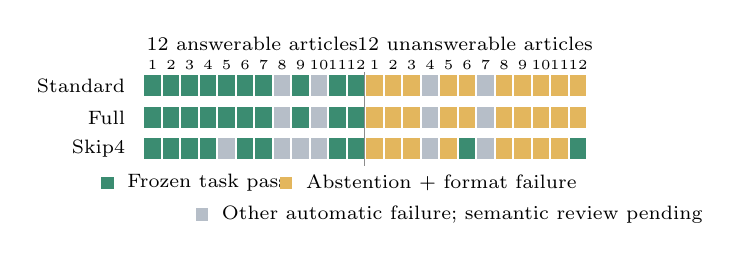
\begin{tikzpicture}[font=\scriptsize]
\node at (1.37,.67) {12 answerable articles};\node at (4.20,.67) {12 unanswerable articles};
\foreach \i in {0,...,23} {\pgfmathtruncatemacro{\n}{mod(\i,12)+1}\node[font=\tiny] at (\i*.235+.104,.40) {\n};}
\node[anchor=east] at (-.12,.13) {Standard};
\node[anchor=east] at (-.12,-.27) {Full};
\node[anchor=east] at (-.12,-.67) {Skip4};
\fill[passgreen] (0.000,0.000) rectangle ++(.208,.27);
\fill[passgreen] (0.235,0.000) rectangle ++(.208,.27);
\fill[passgreen] (0.470,0.000) rectangle ++(.208,.27);
\fill[passgreen] (0.705,0.000) rectangle ++(.208,.27);
\fill[passgreen] (0.940,0.000) rectangle ++(.208,.27);
\fill[passgreen] (1.175,0.000) rectangle ++(.208,.27);
\fill[passgreen] (1.410,0.000) rectangle ++(.208,.27);
\fill[failgray] (1.645,0.000) rectangle ++(.208,.27);
\fill[passgreen] (1.880,0.000) rectangle ++(.208,.27);
\fill[failgray] (2.115,0.000) rectangle ++(.208,.27);
\fill[passgreen] (2.350,0.000) rectangle ++(.208,.27);
\fill[passgreen] (2.585,0.000) rectangle ++(.208,.27);
\fill[formatamber] (2.820,0.000) rectangle ++(.208,.27);
\fill[formatamber] (3.055,0.000) rectangle ++(.208,.27);
\fill[formatamber] (3.290,0.000) rectangle ++(.208,.27);
\fill[failgray] (3.525,0.000) rectangle ++(.208,.27);
\fill[formatamber] (3.760,0.000) rectangle ++(.208,.27);
\fill[formatamber] (3.995,0.000) rectangle ++(.208,.27);
\fill[failgray] (4.230,0.000) rectangle ++(.208,.27);
\fill[formatamber] (4.465,0.000) rectangle ++(.208,.27);
\fill[formatamber] (4.700,0.000) rectangle ++(.208,.27);
\fill[formatamber] (4.935,0.000) rectangle ++(.208,.27);
\fill[formatamber] (5.170,0.000) rectangle ++(.208,.27);
\fill[formatamber] (5.405,0.000) rectangle ++(.208,.27);
\fill[passgreen] (0.000,-0.400) rectangle ++(.208,.27);
\fill[passgreen] (0.235,-0.400) rectangle ++(.208,.27);
\fill[passgreen] (0.470,-0.400) rectangle ++(.208,.27);
\fill[passgreen] (0.705,-0.400) rectangle ++(.208,.27);
\fill[passgreen] (0.940,-0.400) rectangle ++(.208,.27);
\fill[passgreen] (1.175,-0.400) rectangle ++(.208,.27);
\fill[passgreen] (1.410,-0.400) rectangle ++(.208,.27);
\fill[failgray] (1.645,-0.400) rectangle ++(.208,.27);
\fill[passgreen] (1.880,-0.400) rectangle ++(.208,.27);
\fill[failgray] (2.115,-0.400) rectangle ++(.208,.27);
\fill[passgreen] (2.350,-0.400) rectangle ++(.208,.27);
\fill[passgreen] (2.585,-0.400) rectangle ++(.208,.27);
\fill[formatamber] (2.820,-0.400) rectangle ++(.208,.27);
\fill[formatamber] (3.055,-0.400) rectangle ++(.208,.27);
\fill[formatamber] (3.290,-0.400) rectangle ++(.208,.27);
\fill[failgray] (3.525,-0.400) rectangle ++(.208,.27);
\fill[formatamber] (3.760,-0.400) rectangle ++(.208,.27);
\fill[formatamber] (3.995,-0.400) rectangle ++(.208,.27);
\fill[failgray] (4.230,-0.400) rectangle ++(.208,.27);
\fill[formatamber] (4.465,-0.400) rectangle ++(.208,.27);
\fill[formatamber] (4.700,-0.400) rectangle ++(.208,.27);
\fill[formatamber] (4.935,-0.400) rectangle ++(.208,.27);
\fill[formatamber] (5.170,-0.400) rectangle ++(.208,.27);
\fill[formatamber] (5.405,-0.400) rectangle ++(.208,.27);
\fill[passgreen] (0.000,-0.800) rectangle ++(.208,.27);
\fill[passgreen] (0.235,-0.800) rectangle ++(.208,.27);
\fill[passgreen] (0.470,-0.800) rectangle ++(.208,.27);
\fill[passgreen] (0.705,-0.800) rectangle ++(.208,.27);
\fill[failgray] (0.940,-0.800) rectangle ++(.208,.27);
\fill[passgreen] (1.175,-0.800) rectangle ++(.208,.27);
\fill[passgreen] (1.410,-0.800) rectangle ++(.208,.27);
\fill[failgray] (1.645,-0.800) rectangle ++(.208,.27);
\fill[failgray] (1.880,-0.800) rectangle ++(.208,.27);
\fill[failgray] (2.115,-0.800) rectangle ++(.208,.27);
\fill[passgreen] (2.350,-0.800) rectangle ++(.208,.27);
\fill[passgreen] (2.585,-0.800) rectangle ++(.208,.27);
\fill[formatamber] (2.820,-0.800) rectangle ++(.208,.27);
\fill[formatamber] (3.055,-0.800) rectangle ++(.208,.27);
\fill[formatamber] (3.290,-0.800) rectangle ++(.208,.27);
\fill[failgray] (3.525,-0.800) rectangle ++(.208,.27);
\fill[formatamber] (3.760,-0.800) rectangle ++(.208,.27);
\fill[passgreen] (3.995,-0.800) rectangle ++(.208,.27);
\fill[failgray] (4.230,-0.800) rectangle ++(.208,.27);
\fill[formatamber] (4.465,-0.800) rectangle ++(.208,.27);
\fill[formatamber] (4.700,-0.800) rectangle ++(.208,.27);
\fill[formatamber] (4.935,-0.800) rectangle ++(.208,.27);
\fill[formatamber] (5.170,-0.800) rectangle ++(.208,.27);
\fill[passgreen] (5.405,-0.800) rectangle ++(.208,.27);

\draw[black!45] (2.79,-.88)--(2.79,.31);
\fill[passgreen] (-.55,-1.18) rectangle ++(.16,.16);\node[anchor=west] at (-.34,-1.1) {Frozen task pass};
\fill[formatamber] (1.72,-1.18) rectangle ++(.16,.16);\node[anchor=west] at (1.93,-1.1) {Abstention + format failure};
\fill[failgray] (.65,-1.58) rectangle ++(.16,.16);\node[anchor=west] at (.86,-1.5) {Other automatic failure; semantic review pending};
\end{tikzpicture}
\caption{Paired outcomes retain the case identities hidden by equal totals.
Article order within each half follows the frozen cohort. Green is the original
automatic pass; amber is a post-hoc diagnostic for unanswerable cases beginning
with \texttt{unknown} but failing the contract. Gray does not mean proven factual
error: it includes lexical and citation mismatch. Standard/full each pass 10/24;
skip4 passes a different 10/24 and loses two standard-passing cases. No diagnostic
color changes the frozen verdict.}
\label{fig:research-quality}
\end{figure}


The two failures differ. Case 08 expands the correct ``October
1973'' into a sentence about the oil crisis, failing exact-reference scoring
without demonstrating a factual error. Case 16 gives ``pharma'' with the
placeholder citation \texttt{[source\_id:0]}, a real locator failure. The
interpretation must retain that distinction instead of describing both as
hallucinations or dismissing both as metric noise.

On the 12 unanswerable questions, standard produces ten responses beginning
with \texttt{unknown} but with extra/invalid citation text and two unsupported
substantive answers. All fail the strict contract. Ten are not automatically
ten hallucinations. The raw responses and review packet preserve the distinction.
The frozen counts are unchanged. Earlier ten-case development passes therefore
did not establish robust abstention or citation behavior on separate articles.

\subsection{RQ4 Findings: Publication, Answer Time and Prediction Error}
\textbf{The reservation remains after ingestion finishes.} At arrival zero,
E2 shared and 2+2 publication times are 14.2 and 7.5\,s for incremental updates,
and 50.2 and 26.8\,s for rebuilds. New answers finish at 288.5 and 413.7\,s for
incremental updates, and 304.6 and 420.8\,s for rebuilds. These medians cover
three different documents. Shared execution finishes the new answer earlier
in all 12 matched E2 pairs. Publication precedes current completion in all 24
concurrent episodes, but the fixed partition still limits the old and new
requests. Deferring ingestion protects the old request while delaying publication.
We do not test returning the reserved cores to inference after ingestion ends.

\textbf{The timing model has limited predictive value.} E3 correctly predicts
that shared execution is faster than 2+2 in six pairs. Mean absolute error is
2.54\,s for current completion, 0.50\,s for publication and 22.22\,s for new-answer
completion. The last value is a mean relative error of 6.49\% from update
arrival. A simple baseline using each policy's E2 median has an error of
21.48\,s. This baseline was added after E3 and was not part of the frozen
comparison. The phase model does not show better accuracy. In every E3 case,
publication finishes before the new request arrives and the occupied slot
limits progress. We therefore have not tested a boundary between regimes.

All 48 E2/E3 current-answer and retrieval checks pass. Of the new outputs,
32 pass the strict answer contract. These episodes cover six distinct
answerable questions. Two produce longer answers that fail exact matching
across their configurations. Human review is needed to assess their meaning.
The experiments do not test abstention. The earlier application control below uses a sequential arrival rule.

\subsubsection{Earlier Sequential Application Control}
\label{sec:joint}
\paragraph{Publication and answer times.}
All 12 application episodes complete. Current answers pass their supported
checks and retrieval locates the new source in v2 in every episode. Publication and retrieval therefore work in these episodes. We still need
the answer checks to determine whether the new outputs are valid.

\begin{table}[t]
\caption{Median times from update arrival across three matched episode blocks
with different new documents. $T_c$ is current completion, $T_p$ is publication and $T_f$ is new-answer completion. These are descriptive medians, not confidence bounds.}
\label{tab:joint}
\centering
\begin{tabular}{lrrr}
\toprule
Policy & $T_c$ & $T_p$ & $T_f$\\
\midrule
Standard concurrent & 76.2 & 14.7 & 189.8 \\
Standard deferred & 70.7 & 76.0 & 189.0 \\
Full prototype & 78.5 & 10.3 & 198.9 \\
Skip4 prototype & 76.6 & 9.9 & 189.6 \\
\bottomrule

\end{tabular}
\end{table}
The full prototype publishes earlier than standard concurrent (10.3 versus
14.7\,s median), but its current and fresh answers finish later (78.5 versus
76.2\,s for current answers and 198.9 versus 189.8\,s for new answers). Skip4 publishes at 9.9\,s, with fresh completion
189.6\,s, essentially the same scale as standard. It is already ineligible under
the separate-document paired gate. Deferral protects current service (70.7\,s)
but delays publication to 76.0\,s. None satisfies the frozen automatic joint
benefit criterion.

Figure~\ref{fig:research-episode} shows the timing of one measured episode. In every
concurrent episode, publication precedes current-answer completion. Under the
frozen single-slot trace, Equation~\ref{eq:critical-path} is then governed by
current inference and the next request rather than publication. The measured result is that publication is already complete while
current inference remains active, so accelerating publication does not advance
the next request in these episodes. It does not
prove that publication speed is irrelevant for earlier-arriving independent
requests, multiple slots or another workload.
\begin{figure*}[t]
\centering
\begin{tikzpicture}[font=\scriptsize,>=Latex]
\fill[answerblue] (0,.72) rectangle ++(.25,.16);\node[anchor=west] at (.33,.80) {Current inference};
\fill[updatepurple] (3.1,.72) rectangle ++(.25,.16);\node[anchor=west] at (3.43,.80) {Incremental publication};
\fill[freshorange] (7.0,.72) rectangle ++(.25,.16);\node[anchor=west] at (7.33,.80) {New-version inference};
\input{generated/episode-timeline}
\draw[->,black!60] (0,-4.28)--(11.15,-4.28);
\foreach \t in {0,50,100,150,200}{\draw[black!60] (\t*.054,-4.22)--(\t*.054,-4.34);\node[anchor=north] at (\t*.054,-4.37) {\t};}
\node at (5.4,-4.92) {Elapsed seconds since update arrival};
\end{tikzpicture}
\caption{Measured critical path, first predeclared matched episode (Normandy),
not a timeline assembled from unrelated medians. Purple ticks label publication;
right labels mark new-answer completion. Publication precedes current-answer
completion for all concurrent arms, so accelerating publication does not release
the serial inference slot earlier. Deferral instead delays publication until the
current answer, leaving fresh completion similar in this episode. The full
prototype answers ``France'' but emits an invalid citation prefix; its timing
is preserved as a failed task. Dotted gaps are post-gate retrieval/submission.}
\label{fig:research-episode}
\end{figure*}


\paragraph{Answer checks.}
The first two added documents ask about Normandy's country and Southern
California's abbreviation. Standard answers ``France'' and ``SoCal'' with valid
locators. Full prototype's first answer has the correct fact but an extra
\texttt{source\_id:} prefix in the locator, which fails the contract. The third
asks what kind of economy Victoria has. All arms generate a relevant elaboration
containing the gold ``highly diversified'', but fail exact-reference scoring.
The longer answer fails the scoring rule. Human review is needed before
interpreting it as an error in the economic description.

The original all-episode quality gate fails for standard as well as the
candidates. We retain that failed result rather than relax the rule after reading the outputs. Separately, even a more permissive interpretation of that
shared elaboration would not make full prototype dominate the measured latency
vector: it publishes faster while answering later. Timing and answer validity are separate results. A new semantic assessment could change quality labels
but would not change these measured timestamps or establish statistical benefit.

The current response uses old pinned oracle evidence, whereas the new response
uses actual retrieval. We therefore claim a versioned-update prototype with one
retrieved fresh question per episode, not a fully validated production RAG
trace. The workload demonstrates neither domain-specific household deployment
utility nor a real-time service contract. Observed response times are in minutes.


\section{Deployment Implications and Open Research Gaps}
\label{sec:discussion}
\subsection{Choosing What to Change}
Our results suggest checking the bottleneck before choosing an intervention.
A precision change needs evidence that memory prevents the concurrent job
from progressing and that the change makes enough memory available. Execution
changes need a well-configured static backend for comparison. Approximate
methods need checks on individual answers and citations. In each case, the
application measurement must show whether the changed work limits completion.

The costs also differ. Repacking speeds up warm requests against our restricted
configuration, but increases startup time and anonymous memory. A client that
follows citations cannot use a broken locator even when the answer contains
the right number. Faster publication helps only if the request would otherwise
wait for it. A fixed CPU split can protect ingestion and then keep slowing
inference after ingestion finishes. These observations support measuring the
whole episode before adopting a policy.

Some failures came from the implementation, including missing libraries,
transport interruptions and protocol handling. Fixing them makes execution
possible. It does not change a failed experimental result into a successful one.
Other problems came from measurement. Exact matching can reject a correct
but longer answer, and unclear formatting instructions can make citation checks
hard to interpret. Those cases need separate assessment with the original
scores retained.

The mechanisms have their own costs. Changed weights can leave history in the
KV cache that differs from replayed state. Omitted attention leaves missing KV.
Repacking uses more anonymous memory. A resource saving may also occur outside
the work that limits completion. These effects belong in the evaluation.

\subsection{What Still Needs to Be Tested}
The experiments compare backend settings, check separate QA articles and
measure allocation policies. Several questions remain. First, an independent
reviewer must assess which automatic failures are incorrect answers and which
are acceptable elaborations or citation errors. The blinded packet is ready
but has not been reviewed. Second, arrival patterns and service budgets need
to come from the intended application. Selecting them after these results
could favor a policy without showing that it helps a real workload.

A useful intervention must improve a limiting part of the application while
meeting the answer requirements under the same total resources. We have not
shown this for a capacity-limited update or for dynamic core reassignment.
Distribution also needs a reason, such as a placement or capacity constraint,
and a comparison that includes communication costs. A gain on one node cannot
be assumed to carry over to several nodes.

More models, workloads and matched episodes are needed to test how widely
the findings apply. Quantization, repacking, batching and attention dropping
are existing methods. Combining them or finding a null result does not itself
establish a new algorithm. Our contribution remains the evaluation framework and the
allocation behavior measured in this ARM deployment.

\subsection{Reproducibility and Limits}
We retain reports, source and configuration hashes, outputs and the data used
to draw figures. The earlier 112 execution cells, 108 validation cells and
12 application episodes measure different things. They are not 232 independent
replications. E1--E3 add 75 cells, including 48 application episodes over six
questions. The timing test remains in one limiting regime and does not establish
a better predictor.

The application studies use one model and one node. The four-node study has
a different purpose. Medians and task scores do not establish significance,
equivalence or noninferiority. We have not measured energy or completed an
independent semantic review. The artifact is local and has no public badge.
The authors still need to review the evidence, interpretation and bibliography
before submission.

\section{Conclusion}
We implemented an evaluation framework that coordinates inference and document
ingestion, controls CPU allocations, records request and publication events,
and checks answers against the retrieved version and citations. It connects
resource measurements to the time required to answer a question on new evidence.

The proposed methodology makes these problems observable through isolated
controls, independent-arrival episodes and predictions frozen before timing
holdout evaluation. Fixed 2+2 allocation reduces update time but raises prefill
and answer latency, and publication finishes before the current inference slot
is released in every concurrent E2/E3 episode. The predictor ranks the two
policies correctly in six pairs, but its mean absolute error does not improve
on the simple baseline. Answer checks also remain necessary because generated
outputs can fail the strict reference contract even when retrieval succeeds.
\bibliography{references}
\bibliographystyle{mlsys2025}
\end{document}
